\chapter{Bootloader}

In this chapter some fundamental concepts to the functioning of a bootloader will be explained and used in practice to load a
placeholder kernel.

Before we start it should be made clear that everything below applies to 32-bit, x86 architecture processors.
The majority of the following concepts, however, are transferable to other common architectures.

\section{Booting in Real Mode}

Before we can understand the basics of a bootloader an introduction about the Real Mode of x86 processors is necessary.

When the computer turns on the x86 processor automatically enters \textbf{Real Mode}, which poses some significant limitations.
Newer processors still support Real Mode to ensure backward compatibility, although it is now considered obsolete.

When in Real Mode the CPU is running by default in 16-bit mode, meaning we are expected to use 16-bit registers for our operations.
While 32-bit registers are technically still available and can be utilized on newer machines their usage is advised against 
for most beginner applications. Switching to 32-bit Protected Mode is an exception to this, as we will see later.

Another limitation of Real Mode is that we only have access to a specific size of memory. When referring to a memory 
address in Real Mode we use a 20-bit physical addressing. The Physical Address is referred to using a Segment and Offset like this: 
\[
\textbf{PA = Segment} \cdot \textbf{16 + Offset}
\]
The CPU fetches the Segment value from a 16-bit segment register and the Offset value from a 16-bit address register.

Essentially, by using this convention we can only represent numbers that fit in a 5 digit hex. It is also apparent that
there are multiple ways to represent the same address. For example the physical address 0x12345 can be represented 
by 0x1234 and 0x0005, 0x1230 and 0x0045, 0x1200 and 0x0345... and so on. This way of addressing memory limits us to just 
below 1MiB of memory.

It should be made clear that the addresses used in Real Mode refer to physical addresses. This hinders us from protecting
memory and defining its owenership because no process is prohibitted from accessing any memory segments.
This problem could be overcome by using a Global Descriptor Table in Protected Mode, however, for the purpose of this book we 
will adopt virtual memory via paging as a more modern approach. Virtual memory, along with paging, will be discussed later in this 
book but a brief explanation of how it helps with memory safety is given just to clarify why physical addressing is limiting.

When using virtual addresses, our Operating System is responsible of mapping every virtual address to a physical one.
By this mapping, the operating systems ensures that each program has its own range of physical addresses.
When two programs refer to the same virtual memory, very little does it matter, since they are translated into 
totally different physical addresses by the operating system, rendering both unable to access eachothers' memory space.

Having said that, Real Mode is simply inadequate for modern systems. This is why engineers came up with another CPU 
Operation Mode called \textbf{Protected Mode}. In this mode, while there is no virtualization by default, we can 
take advantage of how memory is segmented to protect critical data from the user. This is achieved by defining different 
memory segments with different privileges (ring levels). The CPU decides if a piece of code has the privilages 
it tries to claim. This is determined by the segment through which we are accessing that memory (we will se that in
practice). Memory management and CPU Operating Modes will have chapters of their own later in this book.

\section{The Role Of The Bootloader}

When the computer turns on the first program to take control is the BIOS. Among other things that do not concern us in 
this section, the BIOS transfers control to the bootloader which is then responsible for loading the OS. Modern systems 
use UEFI insted to overcome some limitations of the BIOS but for educational purposes we will focus on BIOS.

First, the BIOS scans the data storage devices. More precisely it checks the first 512 bytes of each one, namely the Master Boot Record 
(MBR), which is the memory a bootloader conventionally resides upon. If the last two bytes of the MBR are the word 0xAA55 the BIOS 
identifies the storage device as a bootable device. The code below demonstrates we can sign the MBR by padding all bytes until byte 510
with zeros and then writing the word 0xAA55 to the last two bytes.

\begin{lstlisting}[caption={MBR Signature}]
    times 510 - ($ - $$) db 0
    dw 0xAA55
\end{lstlisting}

Once the bootable is determined control is transfered to the Stage-1 bootloader, located in the first 446 bytes of the MBR.
In advanced operating systems the Stage-1 bootloader reads the partition table, located in the next 64 bytes of the MBR.
This table contains four entries of 16 bytes each. Each entry describes a partition in the storage device. When the Stage-1
bootloader finds the active (bootable) partition it loads the volume boot sector of that partition (VBR) into memory and transfers
control to it. The VBR contains infromation about the file system of that partition and the next stage of bootloading, which can differ
between operating systems. However, for simplicity, in this chapter we will assume that the Stage-1 bootloader loads the kernel directly 
from the MBR.

Below is a table describing the layout of the MBR.

\begin{table}[h]
    \centering
    \renewcommand{\arraystretch}{1.15}
    \begin{tabular}{|c|c|c|c|}
    \hline
    \textbf{Region} & \textbf{Offset (bytes)} & \textbf{Size} & \textbf{Notes} \\
    \hline
    Boot code \& data & \texttt{0x000}–\texttt{0x1BD} & 446 B & Stage-1 bootloader \\
    \hline
    Partition table entry \#1 & \texttt{0x1BE}–\texttt{0x1CD} & 16 B & Status, CHS/LBA, sectors \\
    \hline
    Partition table entry \#2 & \texttt{0x1CE}–\texttt{0x1DD} & 16 B & Status, CHS/LBA, sectors \\
    \hline
    Partition table entry \#3 & \texttt{0x1DE}–\texttt{0x1ED} & 16 B & Status, CHS/LBA, sectors \\
    \hline
    Partition table entry \#4 & \texttt{0x1EE}–\texttt{0x1FD} & 16 B & Status, CHS/LBA, sectors \\
    \hline
    Boot signature & \texttt{0x1FE}–\texttt{0x1FF} & 2 B & \texttt{Contains the word 0x55AA} \\
    \hline
    \end{tabular}
    \caption{Master Boot Record (512 bytes) layout.}
\end{table}
    
For the bootloader to run the BIOS loads the it from the MBR to the memory address 0x7C00. This address has been
traditionally used by BIOS software to load the bootloader. Bootloader developers assume this is where their 
bootloader will be loaded to ensure compatibility. The address 0x7C00 is ideal since it is way below the 1MiB 
accessible range and still leaves space below it for the interrupt vectors (they will be covered soon).

After control has been transfered to the bootloader it is now its job to load the kernel. In a later section 
we will suggest some techniques to overcome the 512-byte barrier and the limitations of the Real Mode. 

To complete the picture, below is a table describing the layout of a partition table entry.
Some concepts in the table will be explained later in this chapter.

\begin{table}[h]
    \centering
    \renewcommand{\arraystretch}{1.15}
    \setlength{\tabcolsep}{10pt}
    
    \begin{tabular}{|c|c|p{7cm}|}
    \hline
    \textbf{Bytes} & \textbf{Field} & \textbf{Description} \\
    \hline
    Byte 0 & Status & 
    \texttt{0x80} = bootable; \texttt{0x00} = non-bootable. Indicates if this partition is active (bootable). \\
    \hline
    Bytes 1-3 & First CHS & 
    Starting Cylinder-Head-Sector address (legacy BIOS format). Retained for backward compatibility; often ignored. \\
    \hline
    Byte 4 & Type & 
    Partition type identifier (e.g., \texttt{0x0B} = FAT32, \texttt{0x07} = NTFS). \\
    \hline
    Bytes 5-7 & Last CHS & 
    Ending Cylinder-Head-Sector address (legacy). Used by old BIOS systems. \\
    \hline
    Bytes 8-11 & First LBA & 
    Logical Block Address (LBA) of the first sector of the partition. Modern OSes use this instead of CHS. \\
    \hline
    Bytes 12-15 & Total Sectors & 
    Number of sectors in the partition (counted from First LBA). Determines partition size. \\
    \hline
    \end{tabular}
    \caption{Structure of a Partition Table Entry (16 bytes total).}
\end{table}

\section{Utilizing BIOS Interrupts}

Before we can load our kernel we must understand how to interact with the BIOS. The BIOS exposes a set of
interrupts that we can use to perform basic I/O operations.

Interrupts are usually defined as signals sent to the CPU to indicate that an event needs immediate attention.
When an interrupt is triggered the CPU stops what it is doing and executes a handler function to deal with the event.
Interrups are devided into software and hardware interrupts. Software interrupts are triggered by software instructions, 
while hardware are triggered by signals sent by hardware devices.

A very important advantage of using interrupts is that they expose a controllabele interface to interact with critical
hardware. This abstraction not only simplifies the development process and detatches the programming from the hardware
specifics, but also allows for arguement checking before execution. Since security is a major concern is such low-level
operations, this is a very important feature. This concept will be extended after user and kernel modes are introduced.

In our case we will be using software interrupts to request services from the BIOS. Such services include reading from
storage devices, printing to the screen and reading from the keyboard. For example the BIOS interrupt \texttt{0x10}
offers video services.

In order to specify which function of the interrupt we want to use, we can pass parameters through CPU registers.
For example, to print a character to the screen using BIOS interrupt \texttt{0x10} we can use the teletype output function
by setting the \texttt{ah} register to \texttt{0x0E} and the \texttt{al} register to the ASCII value of the character we want
to print. Finally, we can trigger the interrupt using the \texttt{int} instruction.

\begin{lstlisting}[caption={Simple BIOS interrupt call in assembly}]
    mov ah, 0x0E      ; BIOS function: teletype output
    mov al, 'A'       ; Character to print
    mov bh, 0x00      ; Page number
    mov bl, 0x07      ; Text color (white)
    int 0x10          ; Call BIOS video interrupt
\end{lstlisting}

% Give INT 0x10 and INT 0x13 as examples
% Explain IVT and give IVT table layout

\section{LBA vs CHS Addressing}

Before understanding how the bootloader will load our kernel we need to introduce a new addressing
model called \textbf{Cylinder-Head-Sector} (or CHS). As the name states, this model mirrors the concept of physical 
cylinders, heads and sectors traditional hard drives use. 

\begin{figure}[H]
    \centering
    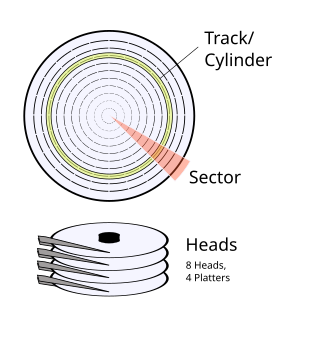
\includegraphics[width=0.4\textwidth]{images/chs_diagram.png}
    \caption{CHS addressing layout: cylinders, heads, and sectors}
    \label{fig:chs}
\end{figure}

As shown above, hard drives are constituted of platters which are essentially circular disks. On both surfaces
of these platters - both top and bottom - data can be written magnetically by a device called head. So for 
4 platters we have 8 heads. 

Now imagine multiple cylinders with centers aligned with the platters'. The intersection of a platter's surface 
and a cylinder is called a track. Naturally we have \(\textbf{Cylinders} \cdot \textbf{Platters} \cdot \textbf{2}\)
number of tracks. Each track can be accessed by only one head.

Each track is divided into sectors, which we can visualize as circular sectors. Each sector defines the smallest addressable
unit upon a track which has a size of 512 bytes.

When writting data to a hard drive we must specify the cylinder, the head and the sector along the track defined by the
cylinder and the head's surface. Each combination of CHS maps to a 512-byte unit or more precisely a Logical Block 
Address (LBA). First, we write data in cylinder 0, head 0, and sector 1 (sectors start counting from number 1). As we 
fill up all sectors up to sector 63 we can start filling up heads. When head 255 is filled, we start filling up cylinders. The 
last available cylinder is 1023. 

\begin{itemize}
    \item \textbf{1024}: Cylinders (0–1023, 10 bits)
    \item \textbf{256}: Heads (0–255, 8 bits)
    \item \textbf{63}: Sectors (1–63, 6 bits), \textit{1-based indexing}
    \item \textbf{512}: Bytes per sector
\end{itemize}

Since CHS is limited at addressing 8.4 GiB of data it has been declared obsolete and replaced by direct LBA addressing.
However, the BIOS still offers this function.

Also, note that modern hard drives do not expose their geometrical structure and instead use an emulation layer for
CHS addressing.

\section{Loading The Kernel}

We can start by dumping some code. Please do not be overwhelmed by it; we will explain it thoroughly shortly after.

\begin{lstlisting}[caption={Simple bootloader start in assembly}]
[ORG 0x7C00] ; This is where the bootloader is loaded in memory
[BITS 16]    ; Bootloader code starts in 16-bit mode

start:
    cli
    mov ax, 0x0700
    mov ss, ax       ; Set stack segment to 0x0700
    mov sp, 0x0000   ; Set stack pointer below of bootloader
    xor ax, ax       ; Zero-out ax
    mov ds, ax       ; Set data segment to 0
    mov es, ax       ; Set extra segment to 0

    mov ah, 0x02
    mov al, 1        ; Number of sectors
    mov ch, 0
    mov cl, 2
    mov dh, 0
    mov dl, 0x80
    mov bx, 0x1000    ; Segment
    mov es, bx
    xor bx, bx        ; Offset
    int 0x13
\end{lstlisting}
    
Let's analyze this line by line. 

First of all, \texttt{cli} is used to prevent the system from triggering maskable interrupts,
requests for the CPU to stop what it is doing and execute some other instructions.
Since interrupt handling has not been set up yet, they will just cause problems.

In lines 6 to 8 we are setting up a simple stack for our Real Mode. To understand these lines we must
remember how physical memory is addressed in Real Mode. It our Stack Segment pointer (ss) we choose segment \texttt{0x0700}
and in our Stack Pointer (sp) we define the offset \texttt{0x0000}. Now the physical address is calculated as such:
\[
\textbf{PA = 0x0700} \cdot \textbf{16 + 0x0000}
\textbf{ => PA = 0x7000 + 0x0000}
\textbf{    => PA = 0X7000}
\]
This address is chosen to be more than 512 bytes below \texttt{0x7C00}, the range where out bootloader is placed.
As mentioned, there are other combinations that could address the same memory as well.
Note that the bootloader might still run without lines 6 to 11, however, without having the stack set up
and the ax, ds and es registers zeroed-out the environment would be highly unpredictable.

Now, being in a controllable environment we can load our kernel into memory. BIOS interrupts will prove useful once again.
In this occasion by calling \texttt{int 0x13} we ask the BIOS to load data from our hard drive into our memory. 
However, before triggering the interrupt we must pass some parameters through CPU registers.

\begin{table}[h]
    \centering
    \begin{tabular}{|c|p{5cm}|p{4cm}|}
    \hline
    \textbf{Register} & \textbf{Purpose} & \textbf{Value Used} \\ \hline
    \texttt{AH} & BIOS function number & \texttt{0x02} (read sectors) \\ \hline
    \texttt{AL} & Number of sectors to read & \texttt{1} sectors \\ \hline
    \texttt{CH} & Cylinder number (part 1) & \texttt{0} \\ \hline
    \texttt{CL} & Sector number (bits 0–5) and high bits of cylinder (bits 6–7) & \texttt{2} (start at sector 2) \\ \hline
    \texttt{DH} & Head number & \texttt{0} \\ \hline
    \texttt{DL} & Drive number & \texttt{0x80} (first hard drive) \\ \hline
    \texttt{ES:BX} & Memory segment:offset where data is stored & \texttt{0x1000:0x0000} (i.e., \texttt{0x10000}) \\ \hline
    \end{tabular}
    \caption{INT 0x13, AH=0x02 — Disk Read BIOS Call Parameters}
    \label{tab:disk_read_params}
\end{table}
    
Since interrupt \texttt{0x13} provides multiple storage device related function we can use the \texttt{ah} register
to choose the \texttt{Read Sectors From Drive} function.
In the \texttt{al} register we can define the number of sectors (512-byte units) we want to read. For simplicity
we will initially be reading just one.

For our case, since the first sector contains the bootloader, we want to start loading from sector number 2.
So we can set our cylinder to 0, our head to 0 and our sector to 2. Be careful when addressing cylinders
as their 2 high bits are defined in bits 6 and 7 of \texttt{cl}.

In the register \texttt{dl} we must specify the storage unit which we want to read data from.
Options \texttt{0x00} to \texttt{0x7F} correspond to floppy discs, while options \texttt{0x80} and higher
correspond to hard drives.

In registers \texttt{es:bx} we use the segment:offset addressing method to specify where in memory we want
to store the data we read.

\begin{lstlisting}[caption={Assembly to load the kernel}]
    mov ah, 0x02
    mov al, 1        ; Number of sectors
    mov ch, 0
    mov cl, 2
    mov dh, 0
    mov dl, 0x80
    mov bx, 0x1000    ; Segment
    mov es, bx
    xor bx, bx        ; Offset
    int 0x13
    jc disk_error   ; Jump if carry flag is set (error occurred)
\end{lstlisting}

After having specified our parameters we can call \texttt{int 0x13} and let the BIOS do its job.

Now, we need to ensure the read operation was conducted successfully. Errors can be detected by checking 
the carry flag. In case of an error the BIOS sets the carry flag. We can use the \texttt{jc} instruction 
to jump to an error handling routine if the carry flag is set. The label \texttt{disk\_error} is defined below.

\begin{lstlisting}[caption={Assembly to handle disk read errors}]
disk_error:
    mov ah, 0x0E
    mov al, 'E'
    int 0x10
    hlt
\end{lstlisting}

This routine uses the teletype output function of the video BIOS interrupt we introduced earlier
to print the character 'E' to the screen, indicating an error has occurred. After printing the error message,
the system halts using the \texttt{hlt} instructionl.

\section{Entering Protected Mode}

A pattern might have started emerging since this is an introductory chapter, but some concepts below are just referred
to and not exllained. Every one of those will be thoroughly explained in next chapters.

Before jumping to our kernel code we will swtich our CPU operating mode from Real Mode to \textbf{Protected Mode}.
Technically, this is not a requirement, however, modern C compilers output 32-bit binaries. To prepare the ground
for our C kernel code properly we will enter Protected Mode before jumping. By doing we enable accessing 4GiB of 
memory as well.

To enter Protected Mode x86 processors require us to have described a memory layout. We can achieve this by defining
a Global Descriptor Table (GDT). Segment selectors can use this table to find their corresponding memory. Since our
approach will use paging for memory management we will set up a very simple GDT in which the code and data segments
overlap just to satisfy the CPU requirement.

\begin{lstlisting}[caption={Defining a GDT}]
gdt_start:
    dq 0x0000000000000000     ; null descriptor
    dq 0x00CF9A000000FFFF     ; code segment
    dq 0x00CF92000000FFFF     ; data segment
gdt_end:

gdt_desc:
    dw gdt_end - gdt_start - 1   ; size = total bytes - 1
    dd gdt_start                 ; address of the GDT
\end{lstlisting}

To pass this table to the CPU we use a descriptor, a pointer to a piece of memory in which we write the size and the 
location of the GDT.

\begin{lstlisting}[caption={Loading GDT and Enabling Protected Mode}]
    lgdt [gdt_desc]
    
    mov eax, cr0
    or eax, 1
    mov cr0, eax

    jmp 0x08:protected_mode_start
\end{lstlisting}

In the snippet above we load the descriptor of the GDT into the CPU and enable the Protected Mode option.
Immediately after, we jump to the \texttt{protected\_mode\_start} label which includes 32 bit mode. We can ignore how and why
we use a far jump and what a far jump is.

Finally, we can tell the assembly compiler we are in 32-bit mode using the \texttt{[BITS 32]} directive and jump
to our kernel. The location of the kernel has been defined when we loaded it from the disk using the int 0x13 instruction.

\begin{lstlisting}[caption={Initializing Registers and Jumping to Kernel}]
[BITS 32]
protected_mode_start:
    ; Set up segment selectors
    mov ax, 0x10
    mov ds, ax
    mov es, ax
    mov fs, ax
    mov gs, ax
    mov ss, ax

    ; Jump to kernel entry point
    jmp 0x08:0x10000
\end{lstlisting}

\section{Build and Run}

TODO

% Compile with nasm
% Create a bootable file
% Run with qemu x86

\section{Two-Stage Bootloaders}

TODO

% Potential additions:
% Segment registers reference table.
% Exercises: load multiple sectors, dump kernel bytes.